\begin{titlepage}
  %\toprule[2pt]
  %\midrule
  \vspace{0.2cm}
  \begin{center}
    \Huge{\textbf{Visualisering af lampers belysning}}
  \end{center}
  \vspace{0.2cm}
  %\midrule
  %\toprule{2pt}
  \vfill
  \begin{center}
  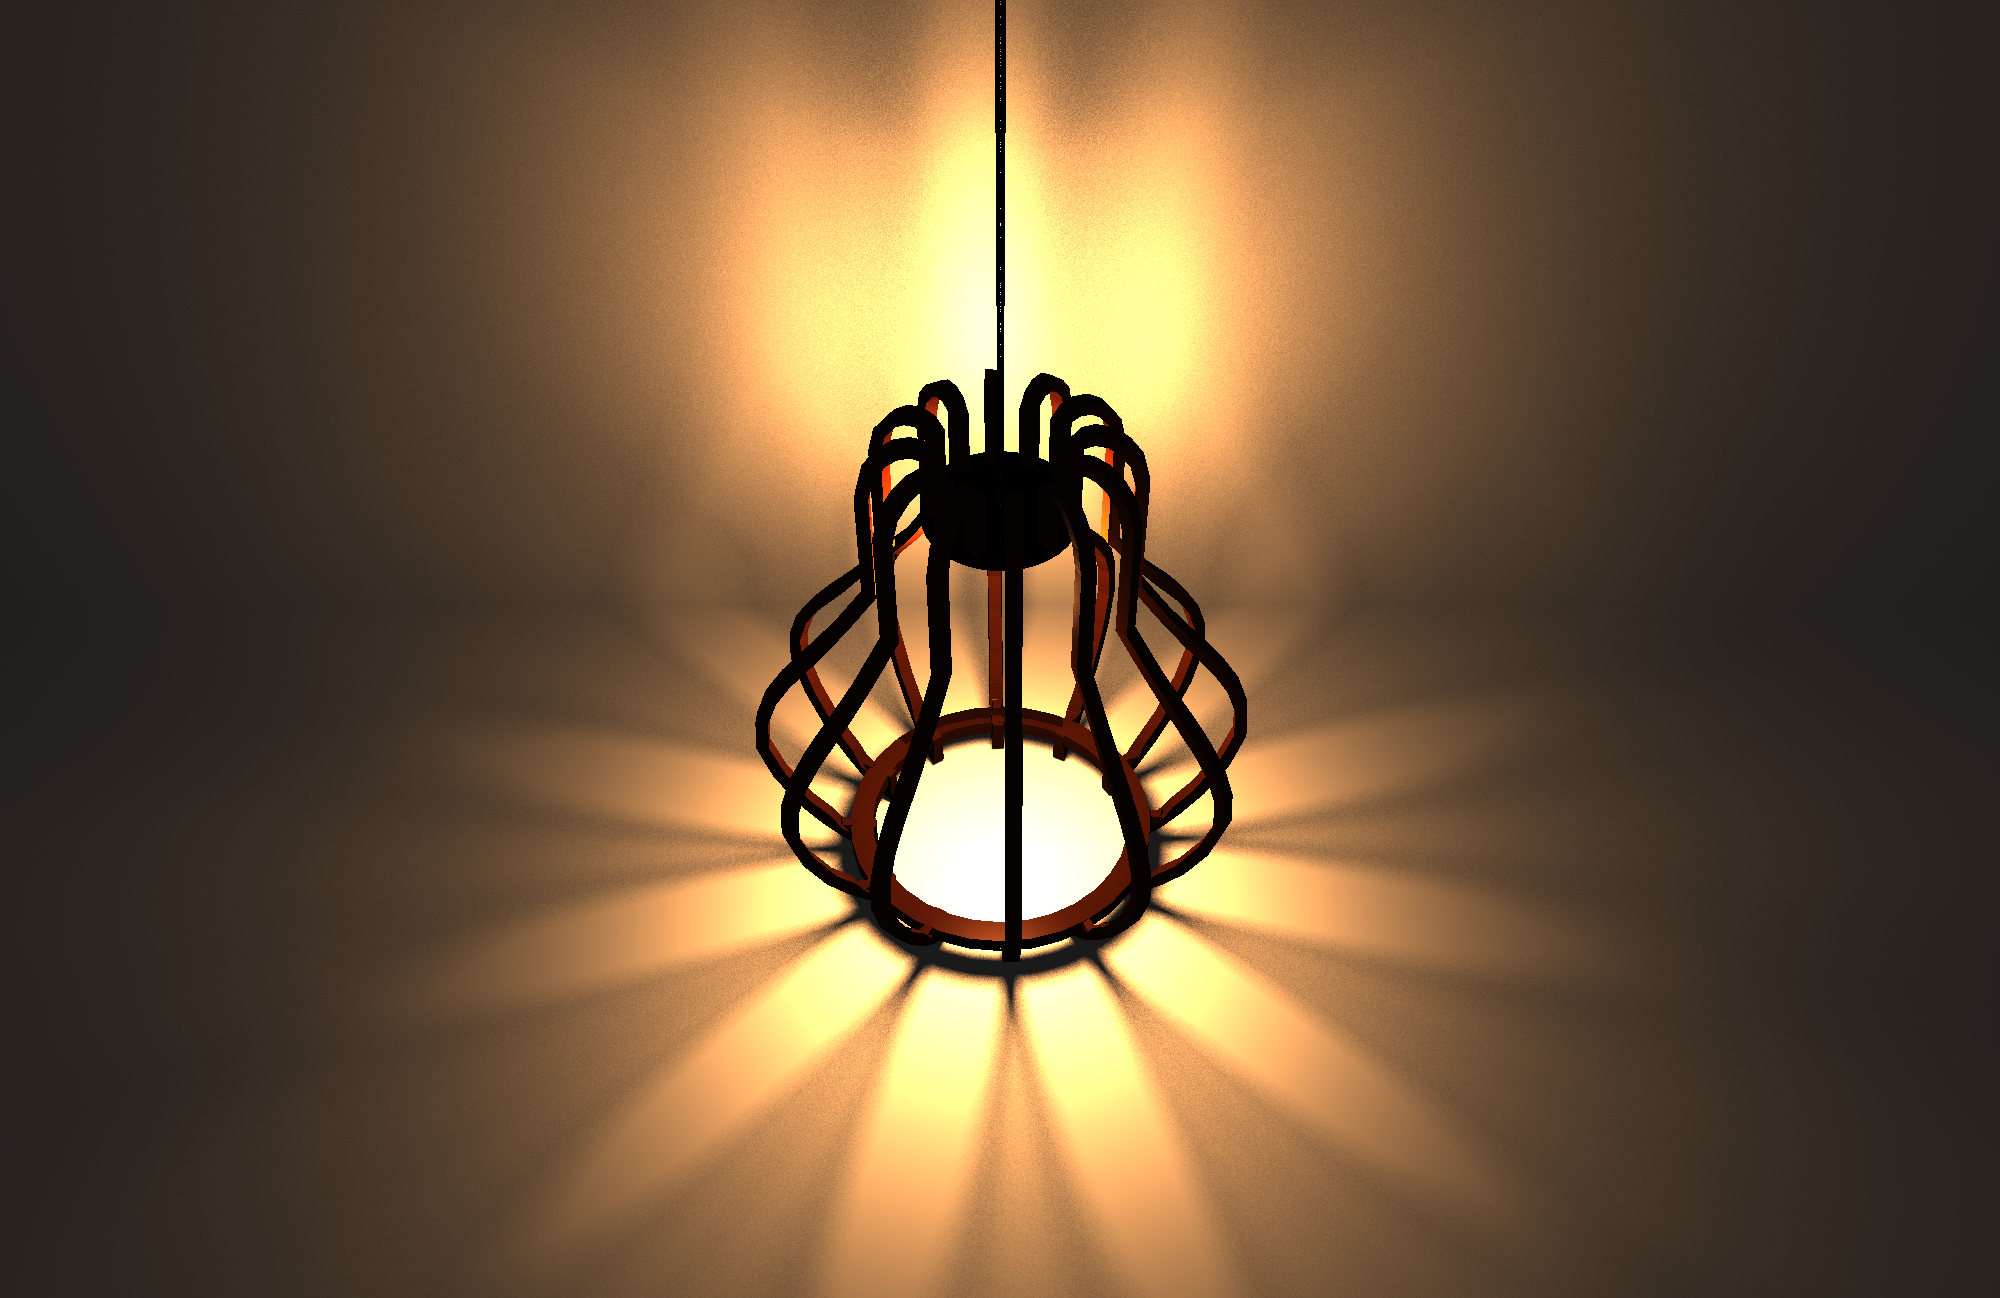
\includegraphics[height=9cm]{front.png}
  \end{center}
  \begin{center}
    \Large{\textbf{Gruppe B2-28}}\\
	Morten Rask Andersen\\
	Anton Christensen\\
	Lasse Fribo Gadegaard\\
	Christian Mønsted Grünberg\\
	Mathias Ibsen\\
	Mathias Rohde Pihl
  \end{center}
  \begin{center}
 	\today\\
    Aalborg Universitet\\
    Software, 1. semester
  \end{center}
\end{titlepage}


%Synopsis
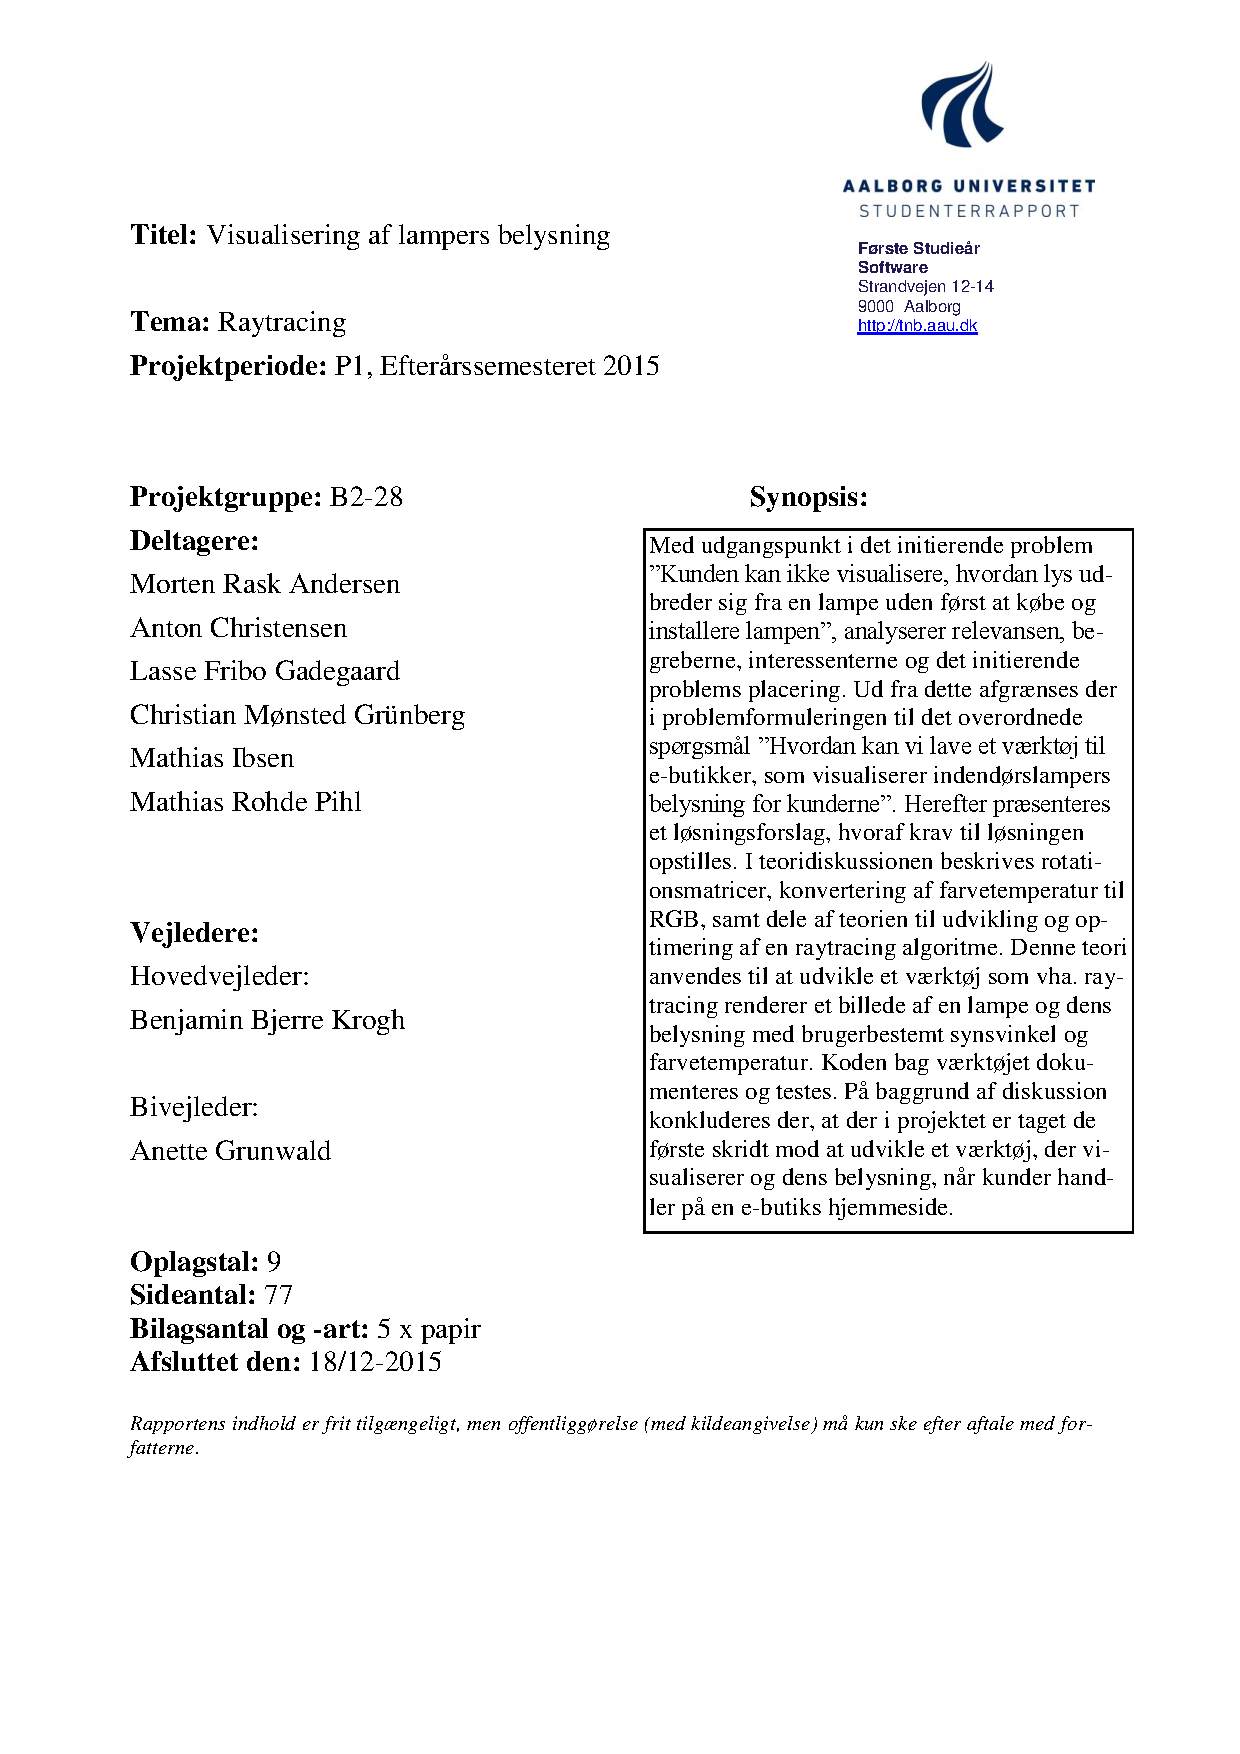
\includepdf[page={-},offset=0mm 0mm]{synopsis_p1}
\addtocounter{page}{-1}
\clearpage

\thispagestyle{empty}
\noindent\begin{tabular}{ll}

\includegraphics[height=1.5cm]{awesome} & 
\includegraphics[height=1.5cm]{a} \\
\makebox[2.5in]{\hrulefill} & \makebox[2.5in]{\hrulefill}\\
Morten Rask Andersen & Anton Christensen\\[8ex]

\includegraphics[height=1.2cm]{las} & 
\includegraphics[height=1.2cm]{chr} \\
\makebox[2.5in]{\hrulefill} & \makebox[2.5in]{\hrulefill}\\
Lasse Fribo Gadegaard & Christian Grünberg\\[8ex]

\includegraphics[height=1.5cm]{ibbe} & 
\includegraphics[height=1.4cm]{pihl} \\
\makebox[2.5in]{\hrulefill} & \makebox[2.5in]{\hrulefill}\\
Mathias Ibsen & Mathias Pihl\\[8ex]
\end{tabular}

\clearpage


\section{Forord}
Denne rapport er udarbejdet af gruppe B2-28, bestående af software-studerende, som P1-rapport på Aalborg Universitet.

Rapporten tager udgangspunkt i Aalborg-modellen for problembaseret læring. Denne læringsproces har givet gruppen mulighed for at undersøge en given problemstilling og derudfra tilegne sig viden, og på baggrund af denne viden udarbejde en problemanalyse. Derudover gør rapporten brug af den kvalitative metode til korrespondance med interessenterne. Den kvalitative metode er fordelagtig at bruge, når man vil undersøge forhold, som er svære at iagttage eller måle \cite{kvalitativ_metode}. I forbindelse med problemanalysen har vi haft kontakt med to lampedesignere og en belysningskonsulent for en dansk lampebutik. Belysningskonsulenten vil efter eget ønske fremgå anonymt. 

Tak til vejledere Benjamin Bjerre Krogh og Annette Grunwald samt den medvirkende belysningskonsulent og de medvirkende designere.

Rapport er blevet afleveret på papirform og online på Digital Eksamen, hvor programmet er blevet vedhæftet. Koden kan derfor findes online og betragtes som elektronisk bilag. Farvede billeder kan derfor også ses på online udgaven af rapporten. 

Som en del af projektet er der i raportens appendiks udarbejdet et projektforslag til næste års P1-forløb.
\clearpage
\subsection{Læsevejledning}
Rapporten er skrevet med en rød tråd, hvilket vil sige, at afsnittene er struktureret således, at der gerne skulle skabes en sammenhæng mellem afsnittene og herefter en helhed. Det er dog ikke nødvendigt at læse hele rapporten, da hvert afsnit har sin egen indledning og opsummering hhv. først og sidst i afsnittet.

Programmet er uploadet til Digital Eksamen og er derfor elektronisk bilag. 

\subsubsection{Kildehenvisning}
Rapportens brug af kildehenvisninger er baseret på nummermetoden \cite{nummermetoden}. I nummermetoden anføres kilderne i fortløbende nummerorden, svarende til hvilket nummer, de har i teksten. To identiske kilder har samme nummer. Herunder ses et eksempel på henvisninger til hhv.\ internetkilder, artikler og bøger:

Interneteksempel med kilde[1].

[1] Titel på emne eller kort forklaring på emnet, hjemmesidenavn. Set DD-MM-YYYY. URL på hjemmeside.


Bogeksempel med kilde[2].

[2] Titel på bog, udgavenummer, forfatter(e), udgivelsesår. ISBN/ISSN-nummer.


Hvis en kilde har yderligere relevante informationer (såsom sidetal, ophavsret mm.\ angives disse også i kilden.


Figurhenvisning foregår på samme måde som med andre kilder, dog med en forklaring under selve figuren. Hvis en figur ingen kilde har, er figuren fremstillet af gruppen.


\subsubsection{Kodeuddrag}
Flere steder i rapporten, vil der blive vist dele af gruppens kode. Et eksempel på hvordan dette vil blive vist er herunder:

\begin{lstlisting}[style=Cstyle, caption=Kodeeksempel i C]
#include <stdio.h>

int main(void){
   printf("Hello, world!\n");
   return 0;
}
\end{lstlisting}

\clearpage